% Probing PostgreSQL with SystemTap and DTrace
\documentclass{beamer}
\usetheme{Berlin}
%\usepackage{tipa}
\usepackage{color}
\usepackage{listings}
\usepackage[utf8,latin9]{inputenc}
\usepackage[T1]{fontenc}
%\usepackage{babel}
\beamertemplatenavigationsymbolsempty

\begin{document}
\title{Probing PostgreSQL with SystemTap and DTrace}
\author{Joshua Tolley -- eggyknap -- End Point Corporation
}

% outline:
% Purpose
%  Sometimes logging isn't enough, and adding extra logging code is certainly not always possible or easy
% Start with DTrace
%  dtrace virtual machine in kernel running bytecode vs. stap compiled to C -> kernel module
%  Mark-based tracing. See -l option
% Show some examples
%  Introduce functions, variables, aggregates, etc. in D
% Show the same thing in systemtap
%  How it works: requires utrace patches for systemtap to do userland. Freebsd doesn't support userland tracing yet
%  Show off mark-based probes
%  Now show off debug-based probes
% Samples / Language introduction
%  sample - Show off some taps / probes while doing this
%  sample - Where am I getting IO, perhaps? What's in cache and what's not?
%  language - Does systemtap have thread-local variables like dtrace does?
% Some advanced stuff
%  Aggregations
% Other usage bits (what tracepoints are there, for instance)

\frame{\titlepage}
%\frame{\tableofcontents}

%\section{The setting}
\begin{frame}
    \frametitle{The problem}
    Sometimes error messages are inadequate
    \begin{figure}[b]
    \begin{centering}
    \scalebox{.75}{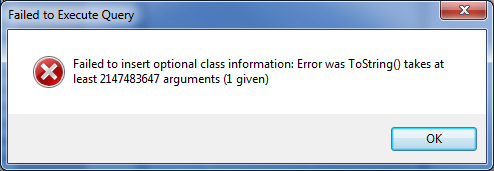
\includegraphics{arguments.png}}
    \end{centering}
    \end{figure}
\end{frame}

\begin{frame}
    \frametitle{The problem}
    Sometimes error logs aren't much better
    \begin{figure}[b]
    \begin{centering}
    \scalebox{.6}{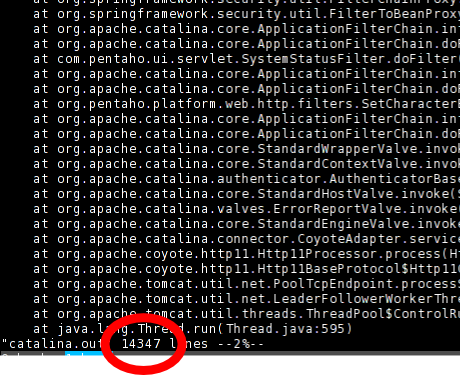
\includegraphics{long_logging_clipped.png}}
    \end{centering}
    \end{figure}
\end{frame}

\begin{frame}
    \frametitle{Typical solutions}
    Often there exists a tool to get the information you're after, but...
    \begin{itemize}
        \item<2->You've never heard of it
        \item<3->No one else has ever heard of it
        \item<4->Even when people *have* heard of it, its options, usage, and output differ completely from the other tools you've used to get to this point, so integration is painful
        \item<5->The more specific the tool, the more output you need to sort through
    \end{itemize}
\end{frame}

%\section{Our hero appears...}
\begin{frame}
    Enter Dynamic Tracing...
\end{frame}

\begin{frame}
    \frametitle{The basics}
    Dynamic tracing allows users to instrument production systems in (ideally) whatever ways they want, without (ideally) breaking things in the process
\end{frame}

%\section{Major players}
\begin{frame}
    \frametitle{The basics}
    Important packages
    \begin{itemize}
        \item<2-> DTrace
        \begin{itemize}
            \item Available on [Open]Solaris, FreeBSD, and OSX
            \item Solaris' version is mature and widely used
            \item FreeBSD's version is less mature than Solaris, and thus has significant limitations
            \item Who runs OSX servers, anyway?
            \item Any guesses how much life OpenSolaris has left?
        \end{itemize}
        \item<3->SystemTap
        \begin{itemize}
            \item Linux only
            \item Less mature than DTrace
            \item Requires kernel tracing patches and/or debug information to be really useful
        \end{itemize}
        \item<4-> There are others (ProbeVue on AIX, other Linux packages with the same goal)
    \end{itemize}
\end{frame}

\begin{frame}
    \frametitle{The basics}
    \begin{itemize}
        \item Software (kernel, libraries, PostgreSQL, etc.) is equipped with various probe points
        \item Simple, C-like scripting language includes variables, functions, screen output, control structures, etc.
        \item User-supplied script describes which probes are used and what to do with them
        \item Compiled and run at the kernel level
        \item Runtime environment includes security and fault tolerance protections
        \item Ideally monitoring overhead is minimal for things that are probed, and nothing for unused probes
    \end{itemize}
\end{frame}

\begin{frame}
     \frametitle{Some differences}
     \begin{itemize}
         \item DTrace compiles to machine code, SystemTap to native code
         \item DTrace is far more mature
         \item SystemTap requires utrace kernel patch (available by default in Fedora, RHEL, CentOS)
         \item SystemTap can put probes anywhere you want, provided you have debug info. DTrace is limited to defined probes and a limited set of other places (function entry/exit, for instance)
         \item DTrace funs on several operating systems, and is CDDL-licensed. SystemTap is Linux only, and GPL
     \end{itemize}
\end{frame}

\begin{frame}
    An example...
\end{frame}

\begin{frame}[fragile]
    "Hello, World!", DTrace style
    \begin{exampleblock}{DTrace script}
    \begin{lstlisting}
BEGIN 
{ 
 trace("Hello, World!"); 
 exit(0); 
}
    \end{lstlisting}
    \end{exampleblock}

    \begin{exampleblock}{Output}
    \begin{verbatim}
dtrace -s Hello.d 
dtrace: script 'Hello.d' matched 1 probe
CPU   ID   FUNCTION:NAME
  0    1      :BEGIN   Hello, World!
    \end{verbatim}
    \end{exampleblock}
\end{frame}

\begin{frame}[fragile]
    \begin{exampleblock}{A more complex example and its output}
    \begin{lstlisting}
syscall:::entry {
    @num[probefunc] = count();
}

  lwp_self                            1
  write                              33
  sigaction                          33
  lwp_sigmask                        53
  ioctl                              95
    \end{lstlisting}
    \end{exampleblock}
\end{frame}

\begin{frame}[fragile]
    \frametitle{Pieces of a DTrace script}
    \begin{itemize}
         \item<1-> Probe declaration (provider:module:function:name). What probe are we looking for?
         \begin{verbatim}
syscall::write:entry
lockstat:::spin-acquire
postgresql1234:::transaction-start
         \end{verbatim}
         \item<2-> Predicate (optional). Are there only certain conditions where this probe is interesting?
         \begin{verbatim}
/execname == "postgres"/
/self->fd = 1/
         \end{verbatim}
         \item<3-> Code to run when probe fires
         \begin{verbatim}
 printf("Hello, world!");
         \end{verbatim}
    \end{itemize}
\end{frame}

\begin{frame}
     These scripts can get extremely complex.
     \begin{itemize}
         \item Thousands or millions of possible probes
         \item Speculative tracing
         \item Aggregates
         \item On-the-fly modification of processes' data
     \end{itemize}
\end{frame}

\begin{frame}[fragile]
     \frametitle{SystemTap}
     SystemTap looks somewhat similar:
     \begin{exampleblock}{SystemTap "Hello, World!"}
     \begin{lstlisting}
probe begin
{
    printf("Hello, World!\n")
    exit()
}
     \end{lstlisting}
     \end{exampleblock}
\end{frame}

\begin{frame}[fragile]
     \begin{exampleblock}{Another example}
     \begin{lstlisting}
probe vfs.read.return {
 if ($return>0) {
  if (devname!="N/A") {
   io_stat[pid(),execname(),uid(),ppid(),"R"]
    += $return
   device[pid(),execname(),uid(),ppid(),"R"]
    = devname
   read_bytes += $return
  }
 }
}
     \end{lstlisting}
     \end{exampleblock}
\end{frame}

\begin{frame}
     That example was part of a much longer script which:
     \begin{itemize}
         \item Captures each filesystem read and write, from each process
         \item Records the process name, device name, operation type, and size
         \item Every five seconds, prints average activity over the five second period, along with statistics for each process that used the disk in that time
     \end{itemize}
\end{frame}

\begin{frame}
     \frametitle{SystemTap script components}
     SystemTap scripts declare a probe and follow it with code, just like DTrace (though SystemTap doesn't support DTrace-style predicates). Probe declarations come in many forms:
     \begin{itemize}
         \item Tapset references -- aliases to other probes, defined in tapset scripts
         \begin{itemize}
             \item \texttt{timer.ms(200)}
             \item \texttt{ioblock.done}
         \end{itemize}
         \item System call probes
         \begin{itemize}
             \item \texttt{syscall.write.begin}
             \item \texttt{syscall.*}
         \end{itemize}
     \end{itemize}
\end{frame}

\begin{frame}
     \frametitle{SystemTap script components}
     \begin{itemize}
         \item Process probes using PID or path to executable
         \begin{itemize}
             \item \texttt{process("/usr/bin/postgres").function("eqjoinsel")}
             \item \texttt{process(31337).function("foo")}
         \end{itemize}
         \item Marker-based probes (allows SystemTap to use defined DTrace probes, without code changes in the application)
         \begin{itemize}
             \item \texttt{process(5783).mark("transaction\_\_start")}
         \end{itemize}
     \end{itemize}
\end{frame}

\begin{frame}
     \frametitle{What can happen inside a probe function?}
     Probes carry with them a set of data. 
\end{frame}

\end{document}
